% !TEX TS-program = lualatex
%\documentclass[handout]{beamer}
\documentclass{beamer}
\input{../common/misomva}
\begin{document}
% Topic-specific title slide
\newcommand{\topictitle}{Small-World Phenomena}
\newcommand{\topicsubtitle}{Erdős Numbers and Disease Spread}
\newcommand{\misoclasstinytitleslide}{Partially based on material by:  Andreas Krause, \\[-1em] Branislav Kveton, Michael Kearns}

\MakeTopicSlide

\begin{frame}
% 
\includegraphics[width=\paperwidth]{img/cgraph}
\end{frame}

\usebackgroundtemplate{%
\tikz\node[opacity=0.10] {%
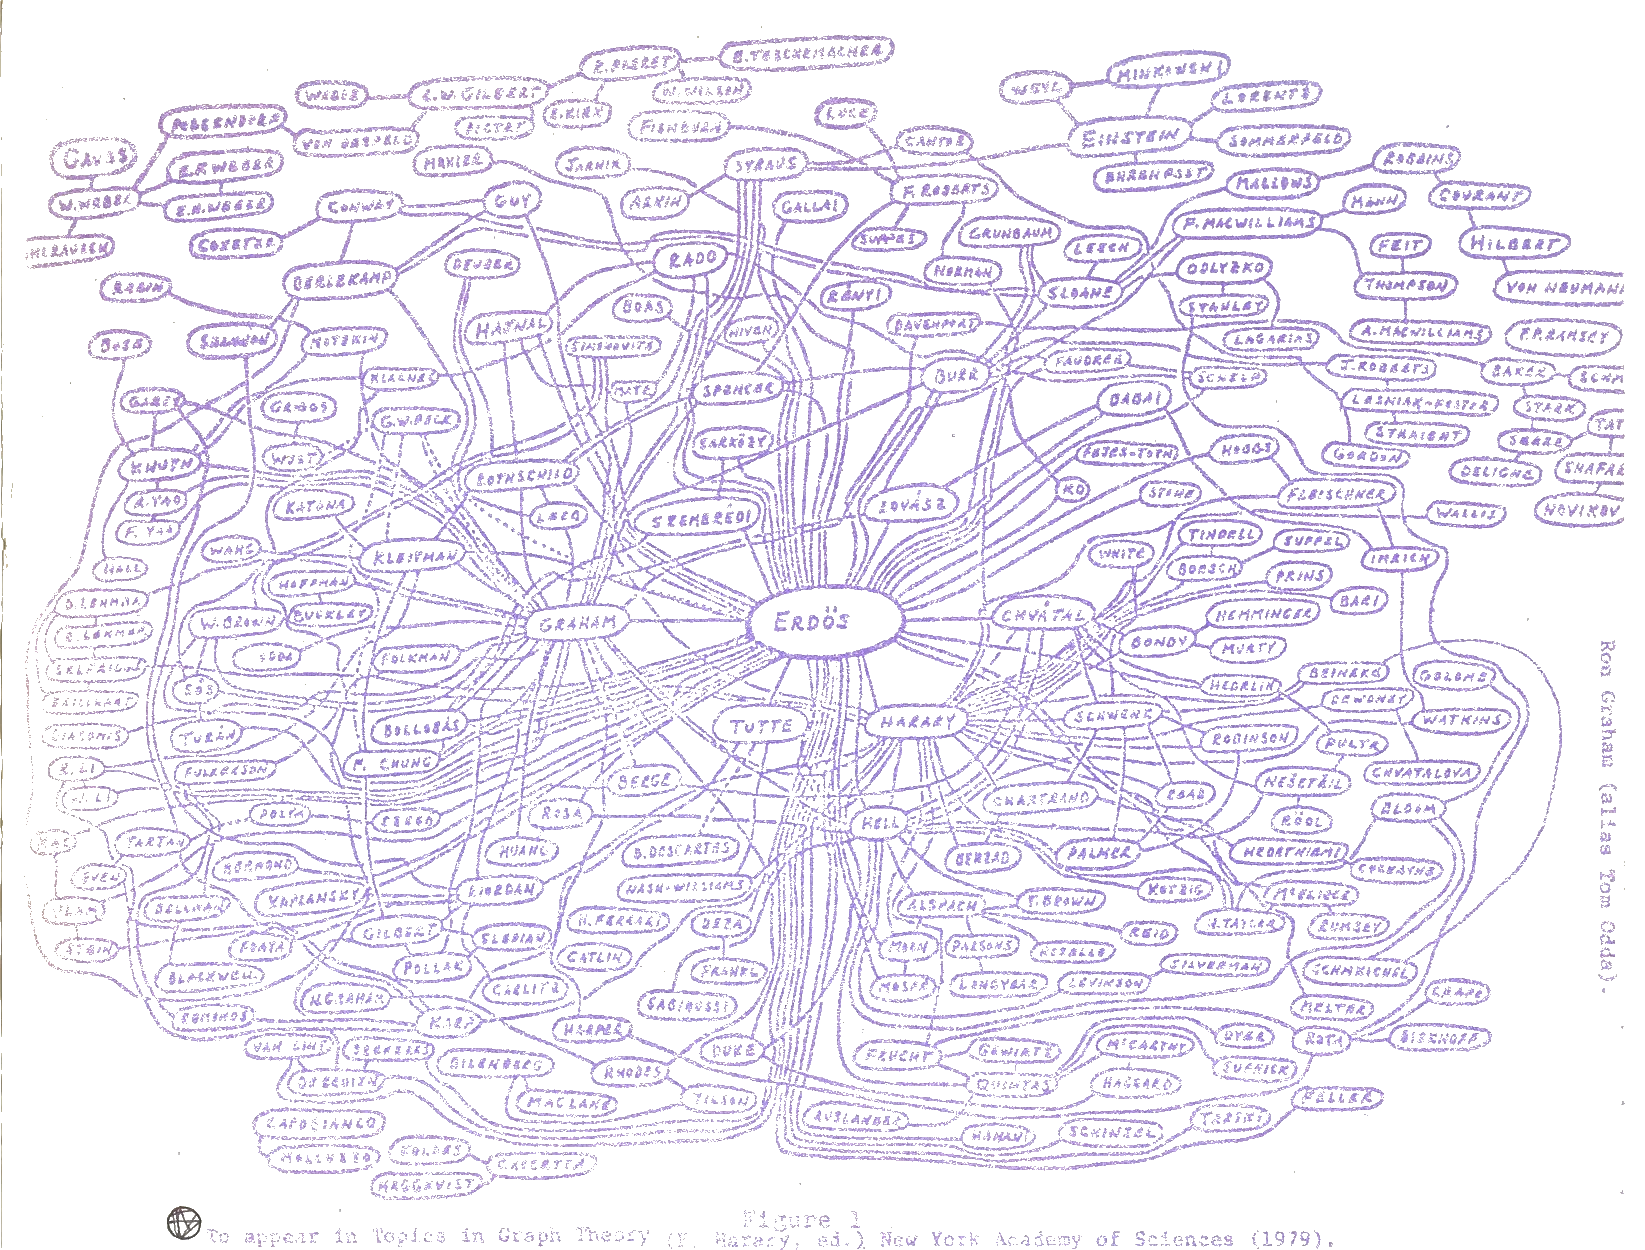
\includegraphics[width=\paperwidth]{../img/cgraph_transparent}
};}

\begin{frame}
\frametitle{Erd\H os number project}
\begin{itemize}[<+-| alert@+>]\addtolength{\itemsep}{0.5\baselineskip}
\item \url{http://www.oakland.edu/enp/} \emphcol{try it!}
\item an example of a real-world graph
\item 401 000 authors, 676 000 edges ($\ll 401000^2 \to$ sparse)
\item average degree 3.36
\item average distance for the largest component: 7.64 
\item 6 degrees of separation [Travers \& Milgram, 1967]
\item heavy tail
\end{itemize}

\end{frame}

\MakeNormalSlide


\begin{frame}
\frametitle{Spanish flu in San Francisco 1918--1919}
\begin{center}

Small-world phenomenon and diseases

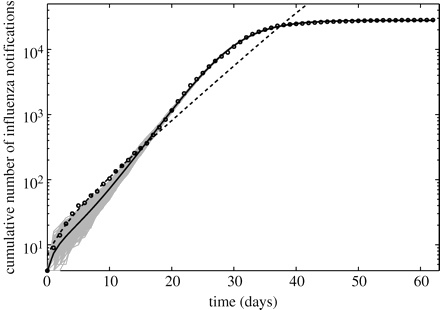
\includegraphics[width=0.75\textwidth]{../img/spanishflu_spread_transparent.png}\moves
{\tiny \url{http://rsif.royalsocietypublishing.org/content/4/12/155}} \moves
\pause
\rightquestionbox{Small world: Obvious?}
\end{center}
\end{frame}




\begin{frame}
\frametitle{Black death!}
\begin{center}
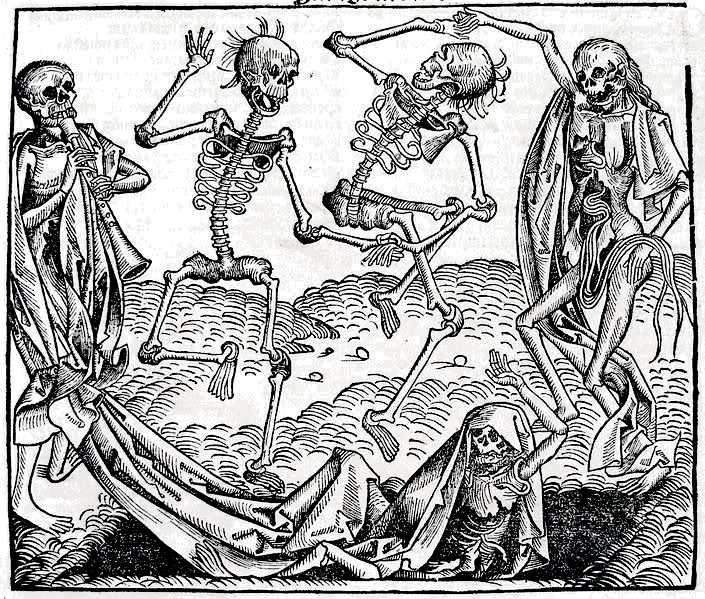
\includegraphics[width=0.75\textwidth]{../img/blackdeath}%\moves
\end{center}
\end{frame}



\begin{frame}
\frametitle{Black death: spread}
\begin{center}

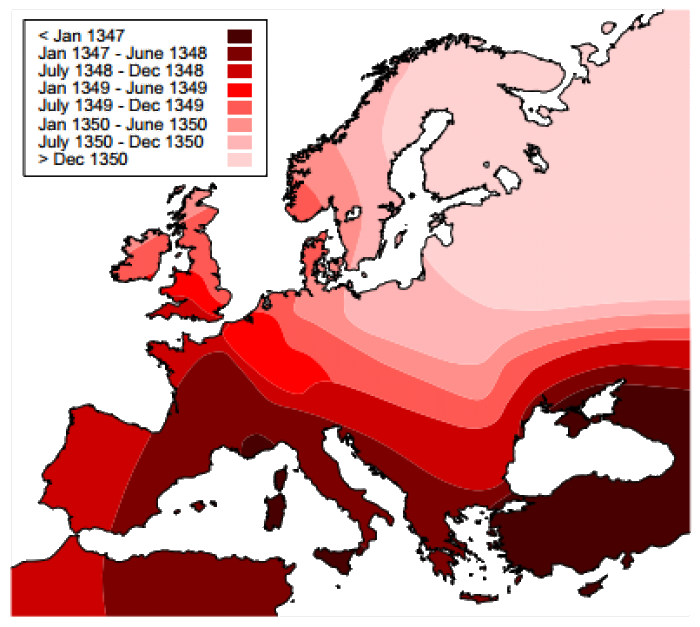
\includegraphics[width=0.60\textwidth]{../img/blackdeath_spread_transparent}\moves
{\tiny source: catholic.org} \moveb

\url{https://www.youtube.com/watch?v=EEK6c9Bh5CQ}
\end{center}
\end{frame}

\MakeLastSlide
\end{document}
